
%! Author = Omar Iskandarani
%! Date = 2025-06-13

% === Metadata ===
\newcommand{\papertitle}{Appendix: Governing Equations of Vorticity in Æther Dynamics}
\newcommand{\paperauthor}{Omar Iskandarani}
\newcommand{\paperaffil}{Independent Researcher, Groningen, The Netherlands}
\newcommand{\paperdoi}{10.5281/zenodo.15566319}
\newcommand{\paperorcid}{0009-0006-1686-3961}

\ifdefined\standalonechapter\else
% Standalone mode
\documentclass[12pt]{article}
\usepackage[a4paper, margin=2cm]{geometry}
\usepackage{ifthen} % we can use it safely now
\usepackage{import}
\usepackage{subfiles}
\usepackage{hyperref}
\usepackage{graphicx}
\usepackage{amsmath, amssymb, physics}
\usepackage{siunitx}
\usepackage{tikz}
\usepackage{booktabs}
\usepackage{caption}
\usepackage{array, tabularx}
\usepackage{listings}
\usepackage{bookmark}
\usepackage{newtxtext,newtxmath}
\usepackage[scaled=0.95]{inconsolata}
\usepackage{mathrsfs}
% vamappendixsetup.sty

\newcommand{\titlepageOpen}{
  \begin{titlepage}
  \thispagestyle{empty}
  \centering
  {\Huge\bfseries \papertitle \par}
  \vspace{1cm}
  {\Large\itshape\textbf{Omar Iskandarani}\textsuperscript{\textbf{*}} \par}
  \vspace{0.5cm}
  {\large \today \par}
  \vspace{0.5cm}
}

% here comes abstract
\newcommand{\titlepageClose}{
  \vfill
  \null
  \begin{picture}(0,0)
  % Adjust position: (x,y) = (left, bottom)
  \put(-200,-40){  % Shift 75pt left, 40pt down
    \begin{minipage}[b]{0.7\textwidth}
    \footnotesize % One step bigger than \tiny
    \renewcommand{\arraystretch}{1.0}
    \noindent\rule{\textwidth}{0.4pt} \\[0.5em]  % ← horizontal line
    \textsuperscript{\textbf{*}}Independent Researcher, Groningen, The Netherlands \\
    Email: \texttt{info@omariskandarani.com} \\
    ORCID: \texttt{\href{https://orcid.org/0009-0006-1686-3961}{0009-0006-1686-3961}} \\
    DOI: \href{https://doi.org/\paperdoi}{\paperdoi} \\
    License: CC-BY 4.0 International \\
    \end{minipage}
  }
  \end{picture}
  \end{titlepage}
}
\begin{document}

    % === Title page ===
    \titlepageOpen

    \begin{abstract}
        This section presents the foundational equations governing vortex dynamics within an incompressible, inviscid fluid, reformulated for the Vortex Æther Model (VAM). Starting from the continuity and momentum equations, we derive vorticity transport laws, Poisson’s equation for scalar potential, and helicity conservation. Particular emphasis is placed on the role of absolute and relative vorticity, external forcing, and height-dependent flows. The resulting barotropic and potential vorticity formulations are essential for analyzing cyclogenesis, turbulence, and topologically conserved quantities in both classical and quantum æther systems. These expressions establish the theoretical infrastructure necessary for modeling swirl-based time dilation, wave-vortex coupling, and rotational energy gradients in vortex-bound matter.
    \end{abstract}

    \titlepageClose
    \fi

% ============= Begin of content ============
    \section{\papertitle}

    The governing equations of vortex dynamics in an idealized fluid system constitute a fundamental framework in contemporary theoretical and applied physics. These equations, rigorously derived from foundational principles in classical mechanics and continuum physics, provide profound insights into a broad spectrum of physical phenomena. By integrating vorticity fields, energy dissipation mechanisms, and entropy dynamics, these formulations extend beyond conventional applications, enabling high-fidelity analyses of macroscopic fluid behaviors and their microscopic analogs within the context of Æther Physics. This synthesis offers an unparalleled theoretical foundation for examining complex interactions, bridging domains from geophysical fluid dynamics to quantum mechanical interpretations of turbulence.

    \begin{table}[H]
        \centering
        \footnotesize
        \renewcommand{\arraystretch}{1.4}
        \begin{tabular}{|c|l|c|c|}
            \hline
            \textbf{Symbol} & \textbf{Description} & \textbf{Unit} & \textbf{VAM Interpretation} \\
            \hline
            $u, v, w$      & Velocity components in $x, y, z$ directions & $\mathrm{m/s}$ & Æther flow vector field \\
            \hline
            $\zeta$        & Relative vorticity $= \frac{\partial v}{\partial x} - \frac{\partial u}{\partial y}$ & $\mathrm{s}^{-1}$ & Local fluid rotation rate \\
            \hline
            $\zeta_a$      & Absolute vorticity $= \zeta + f$ & $\mathrm{s}^{-1}$ & Total vorticity (includes Coriolis) \\
            \hline
            $f$            & Coriolis parameter $= 2\omega \sin(\theta)$ & $\mathrm{s}^{-1}$ & Rotation due to background frame \\
            \hline
            $\omega$       & Planetary or core angular velocity & $\mathrm{rad/s}$ & Frame or vortex rotation rate \\
            \hline
            $\vec{\omega}$ & Vorticity vector field & $\mathrm{s}^{-1}$ & Curl of the velocity field: $\nabla \times \vec{v}$ \\
            \hline
            $R$            & Radius of curvature of streamlines & $\mathrm{m}$ & Local geometric curvature of vortex \\
            \hline
            $V$            & Tangential swirl velocity & $\mathrm{m/s}$ & Clock-hand velocity around vortex \\
            \hline
            $\Pi$          & Potential vorticity $= \frac{f_a + \zeta_r}{h}$ & $\mathrm{s}^{-1}$ & Conserved in barotropic VAM flows \\
            \hline
            $h$            & Column height (layer thickness) & $\mathrm{m}$ & Local æther depth in height-varying flows \\
            \hline
            $\psi$         & Streamfunction ($\zeta = \nabla^2 \psi$) & $\mathrm{m^2/s}$ & Encodes flow via level curves \\
            \hline
            $\phi$         & Scalar potential & $\mathrm{m^2/s^2}$ & Source-based potential (e.g. gravity) \\
            \hline
            $\mathcal{R}_x, \mathcal{R}_y$ & Forcing terms (e.g., turbulence, friction) & $\mathrm{m/s^2}$ & External interaction effects \\
            \hline
            $J(\psi, \nabla^2\psi)$ & Jacobian term & $\mathrm{m^2/s^3}$ & Nonlinear advection in 2D GFD \\
            \hline
            $H = \int \vec{v} \cdot \vec{\omega} \, dV$ & Helicity & $\mathrm{m^4/s^2}$ & Topological twist/linkage of vortex lines \\
            \hline
        \end{tabular}
        \caption{Glossary of symbols used in VAM vortex dynamics equations.}
        \label{tab:vam_vorticity_symbols}
    \end{table}


    \subsection*{Fundamental Equations of Vortex Dynamics}

    \subsubsection*{Continuity Equation}
    \begin{equation*}
        \frac{\partial u}{\partial x} + \frac{\partial v}{\partial y} + \frac{\partial w}{\partial z} = 0
    \end{equation*}
    This equation enforces the incompressibility constraint in ideal fluid dynamics, ensuring conservation of mass. The divergence-free condition of the velocity field is essential for characterizing both naturally occurring and engineered fluid flows, preserving volumetric consistency throughout the domain.

    \subsubsection*{Momentum Conservation}
    \begin{equation*}
        \frac{\partial u}{\partial x} + v \frac{\partial v}{\partial x} + w \frac{\partial w}{\partial x} = \frac{1}{2} \frac{\partial (u^2 + v^2 + w^2)}{\partial x}
    \end{equation*}
    This equation delineates the redistribution of momentum within a dynamic fluid system, elucidating the interplay between velocity gradients and pressure variations.

    \subsubsection*{Definition of Vorticity}
    \begin{align}
        u &= \boldsymbol{x} \omega, \quad \nu=0 \\
        f &= 2 \omega, \quad \zeta=-\alpha \\
        \zeta &= \frac{\partial v}{\partial x} - \frac{\partial u}{\partial y}
    \end{align}
    Vorticity quantifies the local rotational characteristics of a fluid element and serves as a fundamental diagnostic parameter for analyzing turbulence, circulation, and eddy formation.

    \subsection*{Absolute and Relative Vorticity}
    \begin{align}
        \zeta_\text{Absolute} &= f_\text{atom} + \zeta_\text{relative} \\
        f_\text{atom} &= 2 \omega \sin(\theta) \\
        \zeta_{\text {relative }} &=\frac{d v}{d x}-\frac{d u}{d y}
    \end{align}
    Absolute vorticity incorporates planetary rotation effects through the Coriolis parameter and integrates them with local vorticity contributions.

    \subsubsection*{Energy-Entropy Relationship}
    \begin{equation*}
        \Pi = \frac{f_a + \zeta_r}{h}
    \end{equation*}
    This formulation establishes a bridge between vorticity dynamics and thermodynamic fluxes, providing a robust mechanism for quantifying entropy generation.

    \subsection*{Poisson's Equation for Scalar Potential}
    \begin{align}
        \nabla^2 \phi &= -4 \pi \rho \\
        \frac{\delta^2 \phi}{\delta x^2}+\frac{\delta^2 \phi}{\delta y^2}+\frac{\delta^2 \phi}{\delta z^2} &= -4 \pi \rho
    \end{align}
    This equation governs the scalar potential arising from mass density distributions.

    \subsubsection*{Energy and Momentum Conservation in Vortical Systems}
    \begin{align}
        \rho \left( u \frac{\partial u}{\partial x} + v \frac{\partial u}{\partial y} + w \frac{\partial u}{\partial z} - \zeta_\text{atom} v \right) &= -\frac{\partial p}{\partial x} + r_x \\
        p &= \rho g(\eta z)
    \end{align}
    These equations encapsulate the intricate force and momentum interactions within vortex-dominated regimes.


\subsubsection*{Helicity and Topological Constraints}
$H = \int \vec{v} \cdot \vec{\omega} \, dV$
 Helicity, a measure of the linkage and knottedness of vortex lines, serves as a conserved quantity in idealized flows. This conservation underpins the study of topological invariants in fluid mechanics and their extensions into quantum fluids and plasmas.

 \subsubsection*{Vortex Stretching Derivation}

\begin{tcolorbox}[title=Vortex Stretching in Inviscid Æther Flow, colframe=blue!50!black, colback=blue!5!white, coltitle=black, fonttitle=\bfseries, sharp corners=south]
   \begin{figure}[H]
    \centering
    \begin{subfigure}[t]{0.48\textwidth}
        \centering
        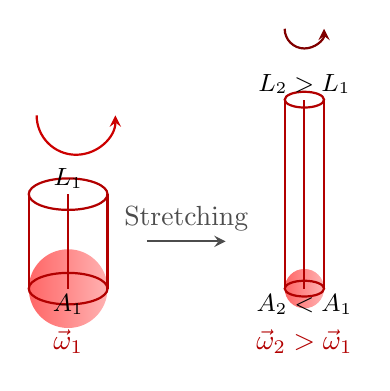
\begin{tikzpicture}[scale=1.0, x={(1cm,0cm)}, y={(0cm,1cm)}, z={(0.3cm,0.2cm)}, >=stealth]
            % Left: initial vortex tube (short & wide)
            \shade[left color=red!60, right color=red!30] (0,0,0) circle (0.5);
            \draw[thick, red!70!black] (0,0,0) ellipse (0.5 and 0.2);
            \draw[thick, red!70!black] (0,0,0) -- (0,1.2,0);
            \draw[thick, red!70!black] (0.5,0,0) -- (0.5,1.2,0);
            \draw[thick, red!70!black] (-0.5,0,0) -- (-0.5,1.2,0);
            \draw[thick, red!70!black] (0,1.2,0) ellipse (0.5 and 0.2);

            \node at (0,-0.2,0) {\small $A_1$};
            \node at (0,1.4,0) {\small $L_1$};
            \node[red!70!black, below] at (0,-0.4) {$\vec{\omega}_1$};

            % Arrow for transformation
            \draw[->, thick, gray!60!black] (1,0.6,0) -- (2,0.6,0) node[midway, above] {Stretching};

             % Front half of the arrow (visible)
            \draw[->, thick, red!80!black]
              (-0.4, 2.2) arc[start angle=180, end angle=360, radius=0.5];

            % Back half (dashed or transparent)
            \draw[->, thick, red!50!black]
              (2.75, 3.3) arc[start angle=180, end angle=360, radius=0.25];

            % Right: stretched vortex tube (tall & thin)
            \shade[left color=red!60, right color=red!30] (3,0,0) circle (0.25);
            \draw[thick, red!70!black] (3,0,0) ellipse (0.25 and 0.1);
            \draw[thick, red!70!black] (3,0,0) -- (3,2.4,0);
            \draw[thick, red!70!black] (3.25,0,0) -- (3.25,2.4,0);
            \draw[thick, red!70!black] (2.75,0,0) -- (2.75,2.4,0);
            \draw[thick, red!70!black] (3,2.4,0) ellipse (0.25 and 0.1);

            \node at (3,-0.2,0) {\small $A_2 < A_1$};
            \node at (3,2.6,0) {\small $L_2 > L_1$};
            \node[red!70!black, below] at (3,-0.4,0) {$\vec{\omega}_2 > \vec{\omega}_1$};
        \end{tikzpicture}
        \caption{Cylindrical representation of vortex stretching.}
        \label{fig:cylinder_vortex_stretching}
    \end{subfigure}%
    \hfill
    \begin{subfigure}[t]{0.48\textwidth}
        \centering
        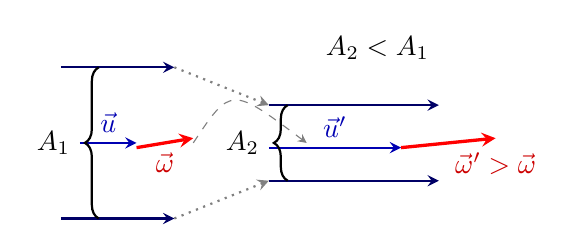
\begin{tikzpicture}[scale=1.2, >=stealth]
            % Left: wide streamlines (converging)
            \draw[->, thick, blue!40!black] (-2,-0.8) -- (-0.8,-0.8);
            \draw[->, thick, blue!40!black] (-2, 0.8) -- (-0.8,  0.8);

            % Transition zone (compression)
            \draw[->, thick, dotted, gray] (-0.8,-0.8) -- (0.2,-0.4);
            \draw[->, thick, dotted, gray] (-0.8, 0.8) -- (0.2, 0.4);

            % Right: narrow streamlines (parallel)
            \draw[->, thick, blue!40!black] (0.2,-0.4) -- (2,-0.4);
            \draw[->, thick, blue!40!black] (0.2, 0.4) -- (2, 0.4);

            % Original vortex filament (shorter)
            \draw[very thick, red, ->] (-1.2,-0.05) -- (-0.6,0.05);
            \node[red!80!black, below] at (-0.9,0) {$\vec{\omega}$};

            % Stretched vortex filament (longer)
            \draw[very thick, red, ->] (1.6,-0.05) -- (2.6,0.05);
            \node[red!80!black, below] at (2.6,0) {$\vec{\omega}' > \vec{\omega}$};

            % Flow velocity vectors
            \draw[->, thick, blue!70!black] (-1.8,0.0) -- (-1.2,0.0) node[midway, above] {$\vec{u}$};
            \draw[->, thick, blue!70!black] (0.2,-0.05) -- (1.6,-0.05) node[midway, above] {$\vec{u}'$};

            % Curved arc to indicate transformation
            \draw[->, dashed, gray] (-0.6,0) .. controls (-0.2,0.6) .. (0.6,0);

            % Area brackets
            \draw[decorate,decoration={brace, amplitude=5pt}, thick] (-1.6,-0.8) -- (-1.6,0.8);
            \node[left] at (-1.8,0) {$A_1$};

            \node[left] at (0.2,0) {$A_2$};
            \draw[decorate,decoration={brace, amplitude=5pt}, thick] (0.4,-0.4) -- (0.4,0.4);
            \node[left] at (2.0,1) {$A_2 < A_1$};
        \end{tikzpicture}
        \caption{Streamline-based view of vortex filament stretching.}
        \label{fig:vortex_stretching_improved}
    \end{subfigure}

    \caption{Two perspectives on vortex stretching in incompressible flow: (a) cylindrical vortex tube conservation, (b) streamline deformation and induced vorticity growth.}
    \label{fig:vortex_stretching_combined}
\end{figure}


In incompressible, inviscid flow, the evolution of vorticity \( \vec{\omega} \equiv \nabla \times \vec{u} \) is governed by deformation of vortex lines due to velocity gradients. Starting from the inviscid Navier--Stokes equation:
\[
\frac{\partial \vec{u}}{\partial t} + (\vec{u} \cdot \nabla)\vec{u} = -\frac{1}{\rho} \nabla p,
\]
we take the curl of both sides:
\[
\frac{\partial}{\partial t} (\nabla \times \vec{u}) + \nabla \times \left[ (\vec{u} \cdot \nabla)\vec{u} \right] = 0.
\]
Recognizing the vorticity \( \vec{\omega} = \nabla \times \vec{u} \), and applying the identity:
\[
\nabla \times \left[ (\vec{u} \cdot \nabla)\vec{u} \right] = (\vec{\omega} \cdot \nabla)\vec{u} - (\vec{u} \cdot \nabla)\vec{\omega},
\]
we derive the vorticity transport equation:
\[
\frac{\partial \vec{\omega}}{\partial t} + (\vec{u} \cdot \nabla)\vec{\omega} = (\vec{\omega} \cdot \nabla)\vec{u},
\]
which simplifies using the material derivative:
\begin{equation}
\boxed{ \frac{D \vec{\omega}}{D t} = (\vec{\omega} \cdot \nabla)\vec{u} }
\end{equation}

\textbf{Interpretation:} The right-hand side represents the \emph{vortex stretching term}. It governs the increase in vorticity magnitude when a vortex filament is stretched by the flow. When a velocity gradient aligns with the direction of vorticity, angular momentum conservation causes the rotation rate to intensify.

\medskip

\textit{Analogy:} Pulling on a spinning elastic band makes it spin faster. Vortex filaments behave similarly under æther flow deformation.

\begin{flushright}
    \textbf{Reference:} G. K. Batchelor, \textit{An Introduction to Fluid Dynamics}, Cambridge University Press, 2000.
\end{flushright}
\end{tcolorbox}


    \subsubsection*{Derivation of Vorticity-Based Fluid Equations}
    The equation:
    \begin{equation*}
        \frac{d u}{d t}+u \frac{d u}{d \boldsymbol{x}}+v \frac{d u}{d y}-\zeta_{\text {atom}} v=-g \frac{d \eta}{d \boldsymbol{x}}+\mathcal{R}_x
    \end{equation*}
    is a form of the \textbf{momentum equation} for the velocity component $u$, incorporating vorticity, gravity effects, and external forcing terms.

    \begin{itemize}
        \item \textbf{Material Derivative} $\frac{d u}{d t}$: Represents the total derivative (substantial derivative) following a fluid parcel.
        \item \textbf{Convective Terms} $u \frac{d u}{dx} + v \frac{d u}{dy}$: Describe how velocity gradients impact acceleration.
        \item \textbf{Vorticity Term} $-\zeta_\text{atom} v$: Arises from the influence of vorticity on velocity evolution.
        \item \textbf{Gravity-Induced Term} $-g \frac{d \eta}{d x}$: Represents pressure gradient due to gravity.
        \item \textbf{External Forcing Term} $\mathcal{R}_x$: Represents additional external forces such as resistive or turbulent effects.
    \end{itemize}

    This equation is derived from the \textbf{Navier-Stokes Equations} under the assumption of an inviscid, incompressible fluid with rotational effects.

    \subsubsection*{Differentiation with Respect to $y$}
    Differentiating the equation with respect to $y$:
    \begin{align}
        \frac{d}{dy} \left( \frac{d u}{d t} + u \frac{d u}{d x} + v \frac{d u}{d y} - \zeta_\text{atom} v \right) &= \frac{d}{dy} \left( - g \frac{d \eta}{d x} + \mathcal{R}_x \right)
    \end{align}
    Expanding this:
    \begin{align}
        \frac{d^2 u}{d t d y}+\frac{d u}{d y} \frac{d u}{d x}+u \frac{d^2 u}{d x d y}+\frac{d v}{d y} \frac{d u}{d y}+v \frac{d^2 u}{d y^2}-\zeta_a \frac{d v}{d y}-\beta v=-g \frac{d^2 \eta}{d x d y}+\frac{d \mathcal{R}_x}{d y}
    \end{align}

    Similarly, differentiating the equation for $v$:
    \begin{equation*}
        \frac{d v}{d t}+u \frac{d v}{d x}+v \frac{d v}{d y}+\zeta_{\text {atom }} u=-g \frac{d \eta}{d y}+\mathcal{R}_v
    \end{equation*}
    Differentiating with respect to $x$:
    \begin{align}
        \frac{d^2 v}{d t d x}+\frac{d u}{d x} \frac{d v}{d x}+u \frac{d^2 v}{d x^2}+\frac{d v}{d x} \frac{d v}{d y}+v \frac{d^2 v}{d x d y}+\zeta_a \frac{d u}{d x}=-g \frac{d^2 \eta}{d x d y}+\frac{d \mathcal{R}_w}{d x}
    \end{align}

    \subsubsection*{Combination of the Two Equations}
    By adding both derived equations, we get:
    \begin{align}
        \frac{\delta \zeta}{\delta t}+\zeta \frac{d u}{d x}+u \frac{\delta \zeta}{\delta x}+\zeta \frac{d v}{d y}+v \frac{\delta \zeta}{\delta y}+\zeta_a\left(\frac{d u}{d x}+\frac{d v}{d y}\right)+\beta v=\frac{d \mathcal{R}_v}{d x}-\frac{d \mathcal{R}_x}{d y}
    \end{align}
    which is a vorticity-based formulation of the original momentum equations.

    \subsubsection*{Representation of Forcing Terms}
    In the presence of external forcing and turbulence:
    \begin{align}
        \mathcal{R}_x &= \frac{1}{\rho}(\tau_x^w - \tau_x^v)
    \end{align}
    \begin{align}
        \mathcal{R}_y &= \frac{1}{\rho}(\tau_y^w - \tau_y^b)
    \end{align}
    where $\tau_x^w, \tau_x^v, \tau_y^w, \tau_y^b$ represent the stress terms.

    \subsubsection*{Final Vorticity Equation}
    \begin{align}
        \frac{D \zeta}{d t}-\frac{\zeta_r+\zeta_a}{h} \frac{D h}{d t}+\frac{D \zeta_a}{d t}=\frac{d R_u}{d x}-\frac{d R_x}{d y}
    \end{align}
    This equation models higher-order vortex interactions, crucial for understanding turbulence, energy dissipation, and wave-vortex interactions.

    \subsubsection*{Conclusion}
    The derivation follows classical fluid dynamics principles and extends into turbulence modeling. These equations are significant in vortex dynamics, superfluid behavior, and atmospheric circulations. They also appear in various studies on vortex ring dynamics.

    \subsubsection*{Governing Vorticity Transport Equation}
    The fundamental vorticity equation is:
    \begin{equation*}
        \frac{\partial \zeta}{\partial t} + u \frac{\partial \zeta}{\partial x} + v \frac{\partial \zeta}{\partial y} + \left( \zeta_r + \zeta_a \right) \left( \frac{\partial u}{\partial x} + \frac{\partial v}{\partial y} \right) + \beta v = \frac{\partial \mathcal{R}_v}{\partial x} - \frac{\partial \mathcal{R}_x}{\partial y}
    \end{equation*}
    where:
    \begin{itemize}
        \item $\zeta$ is the \textbf{relative vorticity}.
        \item $\zeta_r$ and $\zeta_a$ represent \textbf{relative and absolute vorticity contributions}.
        \item $\beta v$ is the \textbf{beta-effect}, modeling the variation of planetary vorticity with latitude.
        \item $\mathcal{R}_x, \mathcal{R}_y$ are external forcing terms, such as frictional forces or turbulence-induced vorticity changes.
    \end{itemize}

    \section*{Vorticity in Height-Dependent Flow}
    \begin{equation*}
        \frac{D \zeta}{d t} - \frac{ \zeta_r + \zeta_a }{h}  \frac{D h}{d t} + \frac{D \zeta_a}{d t}  = \frac{\partial \mathcal{R}_y}{\partial x} - \frac{\partial \mathcal{R}_x}{\partial y}
    \end{equation*}
    This ensures vorticity conservation even in \textbf{variable-height flows}, such as oceanic or atmospheric circulations.

    \subsubsection*{Barotropic Vorticity Equation and Potential Vorticity}
    \begin{equation*}
        D\left(\frac{\zeta_r+\zeta_a}{h}\right)=\frac{1}{h}\left(\frac{d R_y}{d x}-\frac{d R_x}{d y}\right)
    \end{equation*}
    The \textbf{Potential Vorticity (PV)} is conserved:
    \begin{equation*}
        \Pi = \frac{f_a+\zeta_r}{h}
    \end{equation*}
    This is crucial for \textbf{understanding Rossby waves, planetary circulation, and stratified fluid dynamics}.

    \subsubsection*{Relationship to Streamfunction}
    \begin{equation*}
        \zeta = \nabla^2 \psi
    \end{equation*}
    The vorticity field is linked to the \textbf{streamfunction} through the Laplacian operator.

    \subsubsection*{Absolute Vorticity and Coriolis Terms}
    \begin{align}
        f &= 2 \omega, \quad \zeta=-\alpha \\
        f_\text{atom} &= 2 \omega \sin (\theta) \\
        \zeta_\text{Absolute} &= f_\text{atom }+\zeta_\text{relative}
    \end{align}
    Absolute vorticity is the sum of relative vorticity and the Coriolis parameter.

    \subsubsection*{Conservation of Vorticity}
    \begin{equation*}
        \frac{D \zeta}{D t}=0=\frac{\partial \zeta}{\partial t}+u \cdot \nabla \zeta
    \end{equation*}
    In an inviscid flow, vorticity is conserved along streamlines.

    \begin{equation*}
        \frac{\partial \zeta}{\partial t} + u \cdot \nabla(\zeta + f)=0
    \end{equation*}
    \begin{equation*}
        \frac{\partial \zeta}{\partial t}+J(\psi, \nabla^2 \psi)=0
    \end{equation*}
    This is used in \textbf{geophysical fluid dynamics}, where the Jacobian term represents nonlinear advection of vorticity.

    \subsubsection*{Conclusion}
    These equations describe the \textbf{evolution of vorticity in a rotating fluid with height variations and external forcing effects}. They are foundational for:
    \begin{itemize}
        \item Geophysical fluid dynamics (GFD).
        \item Turbulence modeling.
        \item Vortex dynamics in atmospheric and oceanic flows.
    \end{itemize}
    This framework allows for \textbf{wave-vortex interactions}, barotropic/baroclinic instabilities, and the development of \textbf{cyclonic systems}.

% === Bibliography (only for standalone) ===
    \ifdefined\standalonechapter
    % Being imported from main.tex — do nothing
    \else
    \bibliographystyle{unsrt}
    \bibliography{../../references}
    \end{document}
    \fi